%%%%%%%%%%%%%%%%%%%%%%%%%%%%%%%%%%%%%%%%%%%%%%%%%%%%%%%%%%%%%%%%%%%%%%
\section{Casper Design Overview}\label{sec:design}
%%%%%%%%%%%%%%%%%%%%%%%%%%%%%%%%%%%%%%%%%%%%%%%%%%%%%%%%%%%%%%%%%%%%%%

Casper is designed as an external library through the PMPI
name-shifted profiling interface of MPI.  This allows Casper to
transparently link with various MPI implementations, by overloading
the necessary MPI functions.  Casper provides three primary
functionalities: (1) deployment of ghost processes to help with
asynchronous progress, (2) RMA memory allocation and setup, and (3)
redirection of RMA communication operations to appropriate ghost
processes.


%%%%%%%%%%%%%%%%%%%%%%%%%%%%%%%%%%%%%%%%%%%%%%%%%%%%
\subsection{Deployment of Ghost Processes}\label{sec:des-pe}
%%%%%%%%%%%%%%%%%%%%%%%%%%%%%%%%%%%%%%%%%%%%%%%%%%%%

Ghost processes in Casper are allocated in two steps.  In the
first step, when the user launches the application with a number of
processes, a user-defined subset of these processes is carved aside
as the ghost processes at MPI initialization time (see
Figure~\ref{fig:deg-user-comm}).  The remaining processes form their
own subcommunicator called \fn{COMM\_USER\_WORLD}.  The number of
ghost processes is user-defined through an environment variable,
allowing the user to dedicate an arbitrary number of cores on the
node for the ghost processes.

\begin{figure}[htbp]
\centering
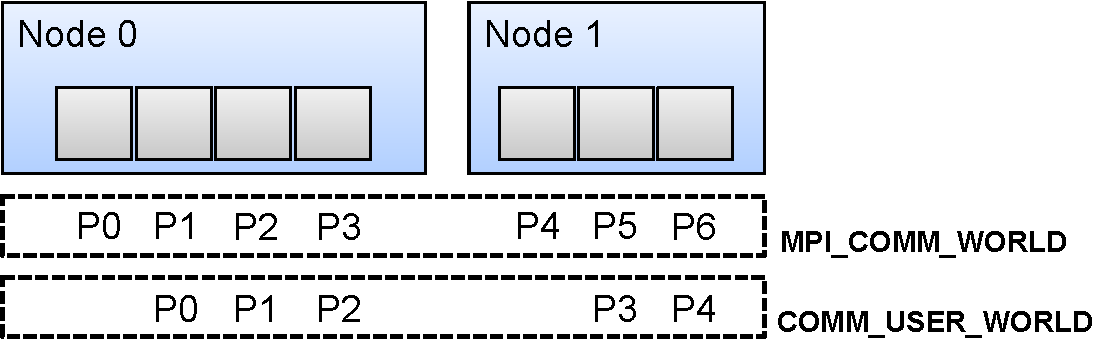
\includegraphics[width=0.9\columnwidth]{figures/casper/design_user_comm.pdf}
\caption{Casper ghost process management.}
\label{fig:deg-user-comm}
% \vspace{-1.0ex}
\end{figure}

In the second step, Casper overrides all MPI operations that take a
communicator argument and replaces any occurrence of
\fn{MPI\_COMM\_WORLD} in all non-RMA functions with
\fn{COMM\_\-USER\_WORLD} at runtime through PMPI redirection.  This
step ensures that all non-RMA communication is redirected to the
correct MPI processes, including creation of other subcommunicators
from \fn{MPI\_COMM\_WORLD}.

After initialization, ghost processes simply wait to receive any
commands from user processes in an \fn{MPI\_RECV} loop.  This approach ensures
that while the ghost processes are waiting for commands, they are
always inside the MPI runtime, thus allowing the MPI implementation to
make progress on any RMA operations that are targeted to those ghost
process.

One aspect to consider in Casper is the locality of application
buffers relative to the ghost processes.  Specifically, since a ghost
process might be depositing or reading data from the application
buffers, how far the ghost process is compared with the buffers can have
a serious impact on performance.  To handle this issue, we ensure that
the ghost processes in Casper are topology-aware.  Casper internally
detects the location of the user processes and places its ghost
processes as close to the application process memory as possible.  For
example, if a node has two NUMA domains and the user requests two
ghost processes, each of the ghost processes places itself in a
different NUMA domain and binds itself to either the process ranks or
segments in that NUMA domain.


%%%%%%%%%%%%%%%%%%%%%%%%%%%%%%%%%%%%%%%%%%%%%%%%%%%%
\subsection{RMA Memory Allocation and Setup}\label{sec:des-init}
%%%%%%%%%%%%%%%%%%%%%%%%%%%%%%%%%%%%%%%%%%%%%%%%%%%%

Remote memory allocation in the Casper architecture is tricky in that
the allocated memory must be accessible by both the application
processes and the ghost processes.  MPI provides two broad
mechanisms to declare a memory region as remotely accessible.  The
first is an ``allocate'' model (i.e., \fn{MPI\_WIN\_ALLOCATE} and
\fn{MPI\_WIN\_ALLOCATE\_SHARED}) in which MPI is responsible for creating
such memory, thus allowing the MPI implementation to optimize such
allocation (e.g., through shared memory or globally symmetric virtual
memory allocation).  The second is a ``create'' model (i.e.,
\fn{MPI\_WIN\_CREATE} and \fn{MPI\_WIN\_CREATE\_DYNAMIC}), in which
the user allocates memory (e.g., using \texttt{malloc}) and then
exposes the memory as remotely accessible.

While memory sharing between the application
processes and the ghost processes can occur in both models, doing so in the
``create'' model requires OS support to expose such capability.  This
capability is generally present on large supercomputers such as Cray
(e.g., through XPMEM~\cite{xpmem} or SMARTMAP~\cite{smartmap}) and
Blue Gene, but not always on traditional cluster platforms.  Thus, for
simplicity, we currently support only the ``allocate'' model.

When the application creates an RMA window using
\fn{MPI\_WIN\_\-ALLOCATE}, Casper follows a three-step process:

\begin{enumerate}

  \item It first allocates a shared-memory region between the user
    processes and the ghost process on the same node using the MPI-3
    \fn{MPI\_WIN\_ALLOCATE\_SHARED} function, as depicted in
    Figure~\ref{fig:deg-mem-map}.  As shown in the figure, the same
    memory region that is used by the application is also mapped onto
    the address space of the ghost process.  Thus, such memory is
    accessible through either process, although care must be taken to
    keep it consistent.

  \item Once the shared memory is allocated, it creates a number of
    internal windows using \fn{MPI\_WIN\_CREATE} to expose this memory
    to all user and ghost processes.

  \item Casper creates a new window with the same memory region
    that contains only the user processes; it then returns the new window
    handle to the application.

\end{enumerate}

\begin{figure}[tbp]
\centering
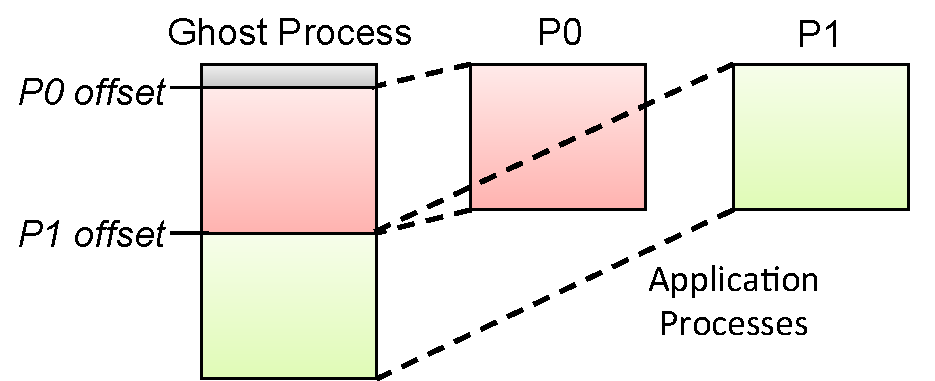
\includegraphics[width=0.7\columnwidth]{figures/casper/design_mem_map.pdf}
\caption{Casper RMA Buffer Mapping}
\label{fig:deg-mem-map}
% \vspace{-3.0ex}
\end{figure}

We note that the Casper architecture exposes the allocated
shared-memory in multiple overlapping windows.  This model provides
Casper's runtime system with enough flexibility to manage permissions
and communication aspects in a highly sophisticated manner; but at the
same time the model requires extreme caution to ensure that memory is not
corrupted and is consistent with the user's expectation.  In
Section~\ref{sec:correctness}, we describe how these internal windows
are utilized in Casper.

%% One subtle, yet important, aspect to be noted here is that the ghost
%% process allocates a slightly larger memory segment as compared to what
%% the user application requires (denoted by the grey box in
%% Figure~\ref{fig:deg-mem-map}).  This extra memory is required for
%% strict compliance with the MPI-3 standard as discussed in more detail
%% in later sections.


%%%%%%%%%%%%%%%%%%%%%%%%%%%%%%%%%%%%%%%%%%%%%%%%%%%%
\subsection{RMA Operation Redirection}\label{sec:des-op}
%%%%%%%%%%%%%%%%%%%%%%%%%%%%%%%%%%%%%%%%%%%%%%%%%%%%

Once the window becomes ready, Casper transparently redirects, through
PMPI redirection, all user RMA operations to the ghost processes on
the target node.  Such redirection needs to translate both the target
rank that the RMA operation is addressed to and the target
offset where the data needs to be written to or read from (since the
offset in the ghost process's memory region might not be the same as
the offset in the user process's memory region).  For example, based on
Figure~\ref{fig:deg-mem-map}, if an origin process does an RMA
operation at offset ``X'' of user process P1, Casper will redirect the
operation to offset ``X + P1's offset in the ghost process address
space'' on the ghost process.

When multiple ghost processes are available on the target node, Casper
attempts to utilize all of them by spreading communication operations
across them.  This approach allows the software processing required for these
operations to be divided between the different ghost processes, thus
improving performance.  Using such a model with multiple ghost processes,
however, requires extra care compared with using a model with a single ghost process. Moreover, it
raises a number of correctness issues, as we discuss
in Section~\ref{sec:multi-ghost}.

%% We note that the shared memory address space on the ghost process is
%% contiguous (see Figure~\ref{fig:deg-mem-map}).  This has both
%% advantages and disadvantages.  The advantage of the contiguous memory
%% address space comes from the offset calculation associated with
%% redirecting RMA operations.  This means that the origin needs to store
%% the offset of each potential target process in the system.  This can
%% be a scalability limitation when scaling to a large number of cores.
%% However, if all of the allocated memory was mapped to a contiguous
%% address space in the ghost process memory, for the common case where
%% all processes allocate the same amount of remotely accessible memory,
%% the origin process would only need to store one offset for each ghost
%% process, rather than one offset for each application process.  Given
%% that the number of ghost processes is expected to be much smaller than
%% the application processes, this can help with scalability concerns.
%% The disadvantage of this approach is that of false sharing.  Since the
%% bordering regions between P0's and P1's memory could be on the same
%% cache line, accesses from P0 and P1 can inadvertently result in
%% additional cache misses compared to the case where Casper was not
%% used.  In this paper, we do not study the performance implications of
%% this design choice in too much detail due to space limitations, but
%% this can be a good aspect to look at for future research.
